\section{Proposed solution} \label{deployment}

    In Fig. \ref{pipeline} we present the main modules of our application. This is a proof of concept for a mobile assistive technology that uses a model of object detection with deep learning, deployed on an Android application. The application can perform object detection on static images and on the live feed from the mobile device's camera, but our main contribution is the accessible live object detection in which the bounding boxes are not drawn on an image, but are converted to text and played on the mobile device speakers. In this way, a VIP could use the application in order to gather information about the environment. We also use an OCR API to provide extra information about the text found in the image, such as the license plate.

    The object detection system is run using the TensorflowLite Task Library, more specifically the object detector that it's already implemented. In order to use this class, the model must be stored in a .tflite file and it must meet some compatibility requirements regarding the input and the output of the model, which are described on the official website \cite{tf_compat}.
    
    %The model is run on a CPU and the number of threads is equal to the available number of CPU cores.
    
       \begin{figure}[!t]
      \centering
      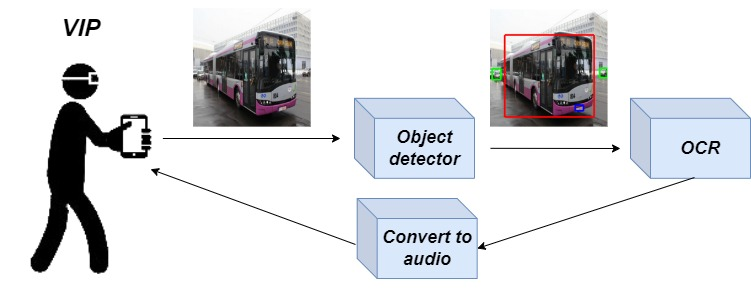
\includegraphics[scale=0.3]{images/pipelinev2.jpg}
      \caption{Step by step pipeline of our solution}
      \label{pipeline}
    \end{figure} 